\documentclass{article}

% packages
\usepackage{amsmath, amsthm, thmtools, amsfonts, amssymb, luacode, catchfile, tikzducks, hyperref, ifthen}
\ifcsname c@kobocompile\endcsname
	\usepackage[a5paper, total={1072pt, 1448pt}, margin=10pt, includeheadfoot]{geometry} % set page margins
\else
	\usepackage[a4paper, margin=50pt, includeheadfoot]{geometry}
\fi
\usepackage[shortlabels]{enumitem}
\usepackage[skip=3pt, indent=0pt]{parskip}

% language
\usepackage[bidi=basic, layout=tabular, provide=*]{babel}
\ifcsname c@english\endcsname
	\babelprovide[main, import]{english}
\else
	\babelprovide[main, import]{hebrew}
	\babelprovide{rl}
\fi
%\babelfont{rm}{Libertinus Serif}
\babelfont{rm}[Renderer=Harfbuzz]{Libertinus Serif}
\babelfont{sf}{Libertinus Sans}
\babelfont{tt}{Libertinus Mono}

% style
\AddToHook{cmd/section/before}{\clearpage}	% Add line break before section
\linespread{1.3}
\setcounter{secnumdepth}{0}		% Remove default number tags from sections, this won't do well with theorems
\AtBeginDocument{\setlength{\belowdisplayskip}{3pt}}
\AtBeginDocument{\setlength{\abovedisplayskip}{3pt}}
\graphicspath{ {../images/} }

% operators
\DeclareMathOperator\cis{cis}
\DeclareMathOperator\Sp{Sp}
\DeclareMathOperator\tr{tr}
\DeclareMathOperator\im{Im}
\DeclareMathOperator\re{Re}
\DeclareMathOperator\diag{diag}
\DeclareMathOperator*\lowlim{\underline{lim}}
\DeclareMathOperator*\uplim{\overline{lim}}
\DeclareMathOperator\rng{rng}
\DeclareMathOperator\Sym{Sym}
\DeclareMathOperator\Arg{Arg}
\DeclareMathOperator\Log{Log}
\DeclareMathOperator\dom{dom}
\DeclareMathOperator\supp{Supp}
\DeclareMathOperator\var{Var}
\DeclareMathOperator\cov{Cov}

% commands
%\renewcommand\qedsymbol{\textbf{מש''ל}}
%\renewcommand\qedsymbol{\fbox{\emoji{lizard}}}
\newcommand{\Aa}[0]{\mathcal{A}}
\newcommand{\Bb}[0]{\mathcal{B}}
\newcommand{\CC}[0]{\mathbb{C}}
\newcommand{\Cc}[0]{\mathcal{C}}
\newcommand{\EE}[0]{\mathbb{E}}
\newcommand{\FF}[0]{\mathbb{F}}
\newcommand{\Ff}[0]{\mathcal{F}}
\newcommand{\Ii}[0]{\mathcal{I}}
\newcommand{\Gg}[0]{\mathcal{G}}
\newcommand{\Ll}[0]{\mathcal{L}}
\newcommand{\Mm}[0]{\mathcal{M}}
\newcommand{\NN}[0]{\mathbb{N}}
\newcommand{\Nn}[0]{\mathcal{N}}
\newcommand{\PP}[0]{\mathbb{P}}
\newcommand{\Pp}[0]{\mathcal{P}}
\newcommand{\QQ}[0]{\mathbb{Q}}
\newcommand{\RR}[0]{\mathbb{R}}
\newcommand{\Rr}[0]{\mathcal{R}}
\newcommand{\Ss}[0]{\mathcal{S}}
\newcommand{\TT}[0]{\mathbb{T}}
\newcommand{\Uu}[0]{\mathcal{U}}
\newcommand{\Vv}[0]{\mathcal{V}}
\newcommand{\Ww}[0]{\mathcal{W}}
\newcommand{\ZZ}[0]{\mathbb{Z}}
\newcommand{\acts}[0]{\circlearrowright}
\newcommand{\explain}[2] {
	\begin{flalign*}
		 && \text{#2} && \text{#1}
	\end{flalign*}
}
\newcommand{\maketitleprint}[0]{ \begin{center}
	%\begin{tikzpicture}[scale=3]
	%	\duck[graduate=gray!20!black, tassel=red!70!black]
	%\end{tikzpicture}	
	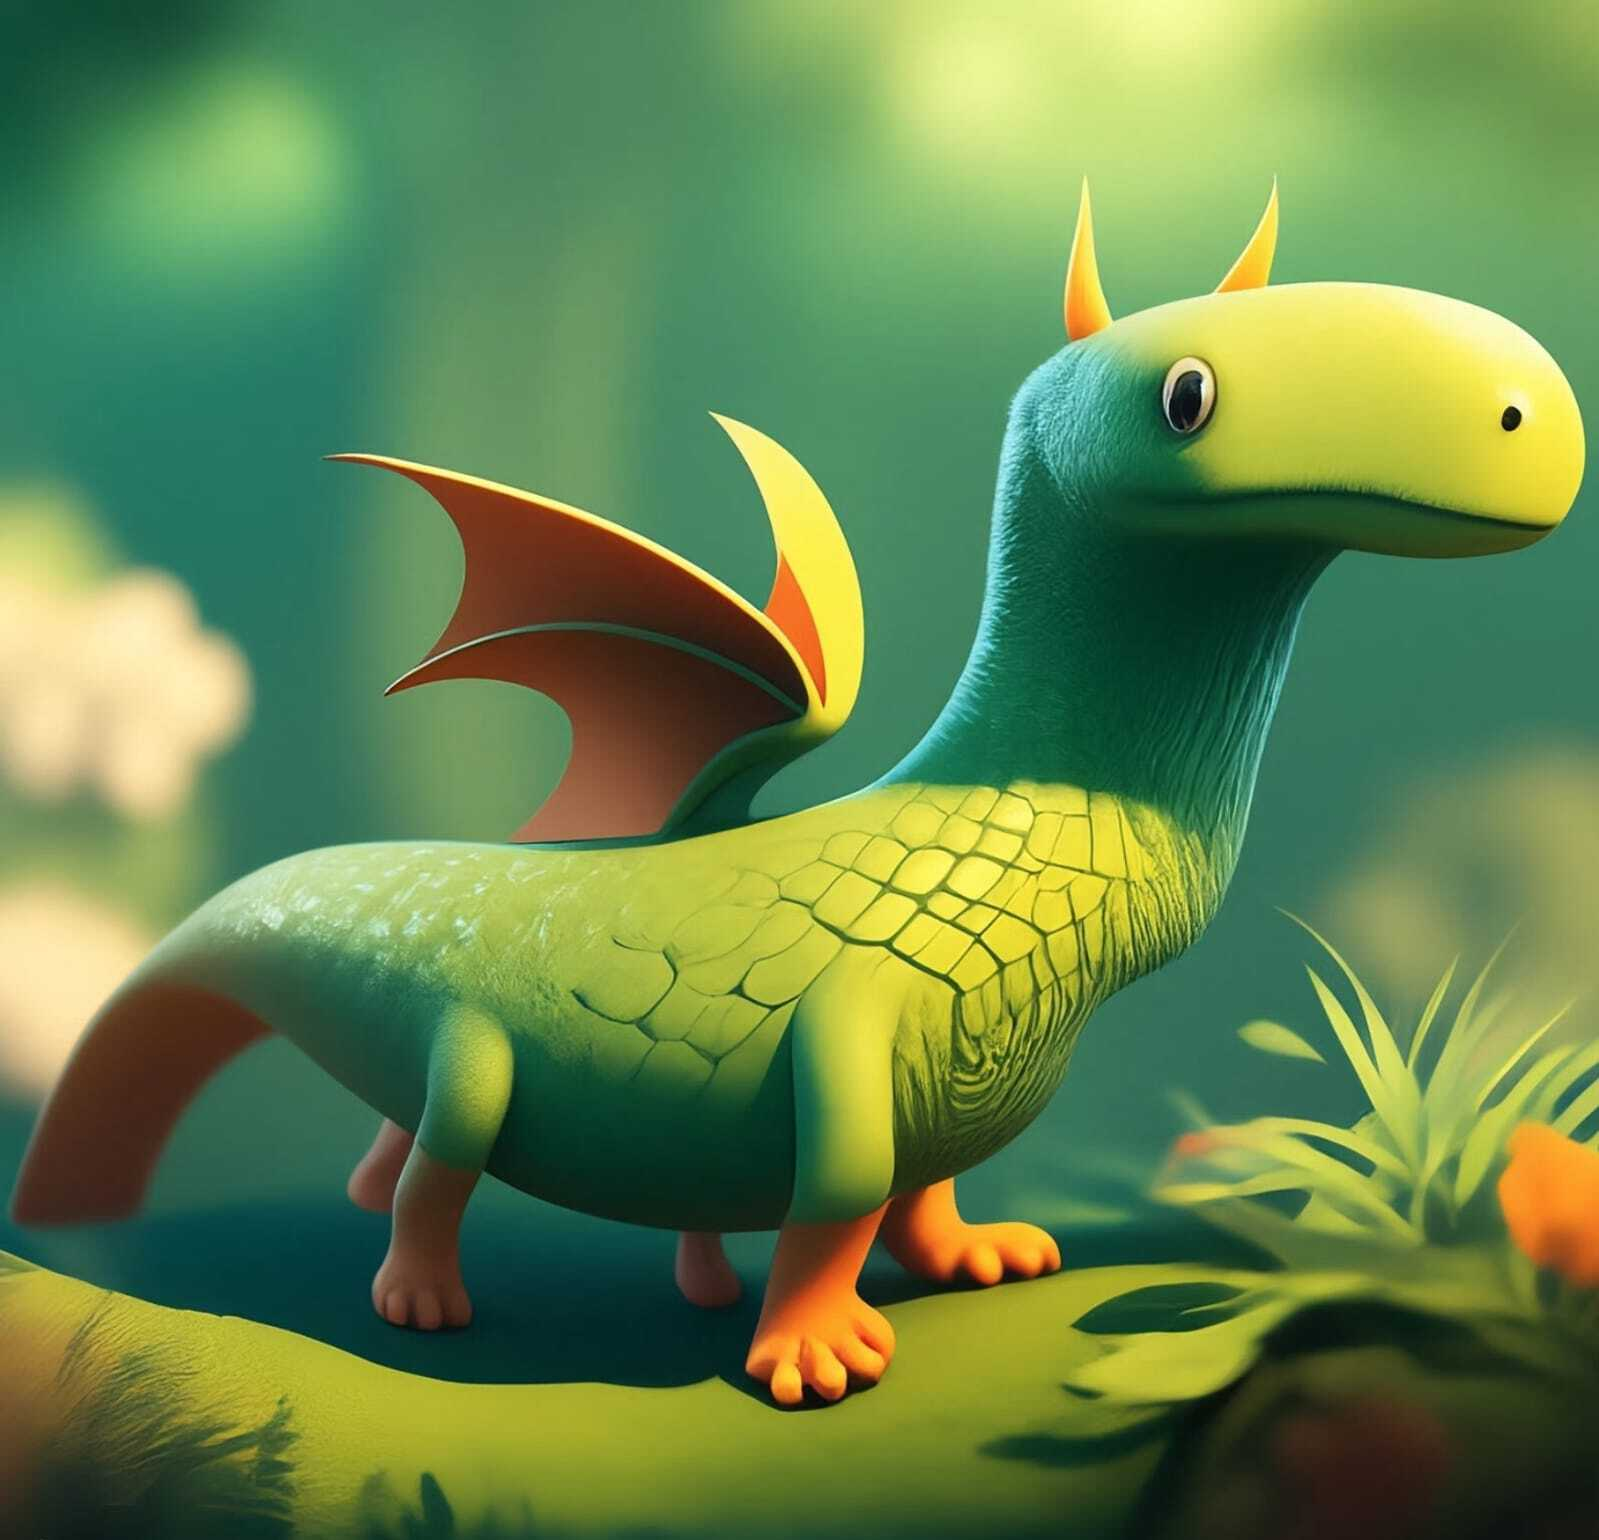
\includegraphics[width=6cm]{cover}
\end{center}
}

% theorem commands
\newtheoremstyle{c_remark}
	{}	% Space above
	{}	% Space below
	{}% Body font
	{}	% Indent amount
	{\bfseries}	% Theorem head font
	{}	% Punctuation after theorem head
	{.5em}	% Space after theorem head
	{\thmname{#1}\thmnumber{ #2}\thmnote{ \normalfont{\text{(#3)}}}}	% head content
\newtheoremstyle{c_definition}
	{3pt}	% Space above
	{3pt}	% Space below
	{}% Body font
	{}	% Indent amount
	{\bfseries}	% Theorem head font
	{}	% Punctuation after theorem head
	{.5em}	% Space after theorem head
	{\thmname{#1}\thmnumber{ #2}\thmnote{ \normalfont{\text{(#3)}}}}	% head content
\newtheoremstyle{c_plain}
	{3pt}	% Space above
	{3pt}	% Space below
	{\itshape}% Body font
	{}	% Indent amount
	{\bfseries}	% Theorem head font
	{}	% Punctuation after theorem head
	{.5em}	% Space after theorem head
	{\thmname{#1}\thmnumber{ #2}\thmnote{ \text{(#3)}}}	% head content

\ifcsname c@english\endcsname
	\theoremstyle{plain}
	\newtheorem{theorem}{Theorem}[section]
	\newtheorem{lemma}[theorem]{Lemma}
	\newtheorem{proposition}[theorem]{Proposition}
	\newtheorem*{proposition*}{Proposition}
	%\newtheorem{corollary}[theorem]{אין חלופה עברית}

	\theoremstyle{definition}
	\newtheorem{definition}[theorem]{Definition}
	\newtheorem*{definition*}{Definition}
	\newtheorem{example}{Example}[section]
	\newtheorem{exercise}{Exercise}[section]

	\theoremstyle{remark}
	\newtheorem*{remark}{Remark}
	\newtheorem*{solution}{Solution}
	\newtheorem{conclusion}[theorem]{Conclusion}
	\newtheorem{notation}[theorem]{Notation}
\else
	\theoremstyle{c_plain}
	\newtheorem{theorem}{משפט}[section]
	\newtheorem{lemma}[theorem]{למה}
	\newtheorem{proposition}[theorem]{טענה}
	\newtheorem*{proposition*}{טענה}
	%\newtheorem{corollary}[theorem]{אין חלופה עברית}

	\theoremstyle{c_definition}
	\newtheorem{definition}[theorem]{הגדרה}
	\newtheorem*{definition*}{הגדרה}
	\newtheorem{example}{דוגמה}[section]
	\newtheorem{exercise}{תרגיל}[section]

	\theoremstyle{c_remark}
	\newtheorem*{remark}{הערה}
	\newtheorem*{solution}{פתרון}
	\newtheorem{conclusion}[theorem]{מסקנה}
	\newtheorem{notation}[theorem]{סימון}
\fi

% Questions related commands
\newcounter{question}
\setcounter{question}{1}
\newcounter{sub_question}
\setcounter{sub_question}{1}

\ifcsname c@english\endcsname
	\newcommand{\question}[1][0]{
		\ifthenelse{#1 = 0}{}{\setcounter{question}{#1}}
		\section{Question \arabic{question}}
		\addtocounter{question}{1}
		\setcounter{sub_question}{1}
	}

	\newcommand{\subquestion}[1][0]{
		\ifthenelse{#1 = 0}{}{\setcounter{sub_question}{#1}}
		\subsection{Part \alph{sub_question}}
		\addtocounter{sub_question}{1}
	}
\else
	\newcommand{\question}[1][0]{
		\ifthenelse{#1 = 0}{}{\setcounter{question}{#1}}
		\section{שאלה \arabic{question}}
		\addtocounter{question}{1}
		\setcounter{sub_question}{1}
	}

	\newcommand{\subquestion}[1][0]{
		\ifthenelse{#1 = 0}{}{\setcounter{sub_question}{#1}}
		\subsection{סעיף \localecounter{letters.gershayim}{sub_question}}
		\addtocounter{sub_question}{1}
	}
\fi

% import lua and start of document
\directlua{common = require ('../common')}

\GetEnv{AUTHOR}

% headers
\author{\AUTHOR}
\date\today

\title{פתרון מטלה 03 --- תורת ההסתברות (1), 80420}

\begin{document}
\maketitle
\maketitleprint{}

\Question{}
נאמר שמאורע $A$ מחזק את מאורע $B$ אם $\PP(B \mid A) > \PP(B)$. \\*
יהי $(\Omega, \PP)$ מרחב הסתברות, ונוכיח או נפריך את הטענות הבאות.

\Subquestion{}
נסתור את הטענה כי אם $A$ מחזק את $B$ ו־$B$ מחזק את $C$, אז $A$ מחזק את $C$, על־ידי דוגמה נגדית.
\begin{solution}
	נניח $\Omega$ הטלת שתי קוביות הוגנות, נניח גם $A$ המאורע שיצא 2 בקוביה הראשונה, $B$ המאורע שיצא 2 לפחות בכל קוביה, ו־$C$ המאורע שיצא לפחות 2 בקוביה ב'. \\*
	נחשב $\PP(B \mid A) = \frac{5}{6} > \PP(B) = \frac{5^2}{6^2}$, בנוסף $\PP(C \mid B) = 1 > \PP(C) = \frac{5}{6}$ אבל $\PP(C \mid A) = \frac{5}{6} = \PP(C) = \frac{5}{6}$.
\end{solution}

\Subquestion{}
נוכיח כי אם $A$ מחזק את $B$ אז גם $B$ מחזק את $A$.
\begin{proof}
	ישירות מהגדרה
	\[
		\PP(B \mid A) > \PP(B)
		\iff \frac{\PP(A \cap B)}{\PP(A)} > \PP(B)
		\iff \frac{\PP(A \cap B)}{\PP(B)} > \PP(A)
		\iff \PP(A \mid B) > \PP(A)
	\]
\end{proof}

\Subquestion{}
נסתור את הטענה כי אם $A, B$ מאורעות המקיימים $\PP(A \cap B) = 0$ אז $A \cap B = \emptyset$.
\begin{solution}
	יהי $\Omega$ הטלת מטבע טריק, מטבע שבו תמיד צד א' נבחר. \\*
	נגדיר גם $A = \Omega$ ו־$B$ מאורע שיצא צד ב', אז כמובן $\PP(A \cap B) = \PP(B) = 0$, אבל $A \cap B$ הוא המקרה שיצא צד ב', ובפרט איננו מאורע ריק.
\end{solution}

\Subquestion{}
נסתור את הטענה כי אם $A, B, C$ מאורעות כך ש־$\PP(A \cap B \cap C) = 0$ וגם $\PP(A \cap B) = 0$ אז $\PP(A \cap C) = 0$.
\begin{solution}
	נגדיר $\Omega = \{0, 1\}$ עם $\PP$ אחידה, ונגדיר $A = C = \Omega, B = \emptyset$, אז נקבל ש־$A \cap B \cap C = A \cap B = \emptyset$ וגם כי $A \cap C = \Omega$, ולכן הטענה מתקיימת.
\end{solution}

\Subquestion{}
נסתור את הטענה כיאם $(\Omega, \PP)$ מרחב הסתברות אחידה, ונניח גם $B$ מאורע כך ש־$\PP(B) > 0$, אז $(\Omega, \PP_B)$ מרחב הסתברות אחידה.
\begin{solution}
	נבחן מרחב הסתברות של הטלת קוביה הוגנת, הוא עומד בכל התנאים, ואם $B = \{ 1, 2, 3 \}$ אז $\PP_B(\{1\}) = \frac{1}{3} \ne 0 = \PP_B(\{4\})$, דהינו מרחב ההסתברות $(\Omega, \PP_B)$ לא אחיד. \\*
	נבחין כי $(\Omega \cap B, \PP_B)$ הוא כן מרחב הסתברות אחיד.
\end{solution}

\Subquestion{}
נוכיח שאם $(\Omega, \PP)$ מרחב הסתברות לא אחיד ויהי $B$ כך ש־$\PP(B) > 0$, אז $(\Omega, \PP_B)$ מרחב הסתברות לא אחיד.
\begin{proof}
	מהנתון נסיק כי $\Omega$ לא ריק, ונבחין בין שני מקרים. \\*
	אם $\Omega = B$ אז $\PP = \PP_B$ ולכן סיימנו. \\*
	אחרת נגדיר $A = \Omega \setminus B$ ולכן $\PP_B(B) = 1 \ne 0 = \PP_B(A)$, ולכן מרחב ההסתברות הוא לא אחיד.
\end{proof}

\Question{}
\Subquestion{}
בשידה שלוש מגירות, באחת זוג גרביים שחור, בשנייה זוג גרביים לבן, ובשלישית גרב שחור וגרב לבן. \\*
בוחרים מגירה באקראי ובהסתברות אחידה ומוציאים ממנה גרס יחיד באקראי, ונתון כי הוא לבן. \\*
מה ההסתברות שגם הכרב השני במגירה לבן?
\begin{solution}
	השאלה שקולה לשאלה מה הסיכוי להוציא גרב לבן ואז גרב לבן נוסף, נגדיר $\Omega = \{ (w, w), (b, b), (w, b), (b, w) \}$. \\*
	נגדיר $A = \{ (w, w), (w, b) \}$ המאורע שהגרב הראשון שנבחר הוא לבן, עוד נבחין כי $p(w, w) = p(b, b) = p(w, b) + p(b, w)$ ו־$p(w, b) = p(b, w)$. \\*
	נגדיר $B = \{ (w, w) \}$ המאורע ששני הגרביים לבנים, ואנו מחפשים את $\PP(B \mid A)$, לכן
	\[
		\PP(B \mid A) = \frac{\PP(A \cap B)}{\PP(A)} = \frac{\PP(B)}{\PP(A)} = \frac{\frac{1}{3}}{\frac{1}{3} + \frac{1}{6}} = \frac{2}{3}
	\]
\end{solution}

\Subquestion{}
נתון דלי עם $k$ כדורים לבנים ו־$k$ כדורים שחורים.
מוציאים $n < k$ כדורים ללא החזרה ולאחר מכן מוציאים כדור נוסף, כדור $n + 1$.
נחשב מה ההסתברות אם ידוע ש־$n$ הכדורים הראשונים לבנים, מה ההסתברות שהכדור ה־$n + 1$ שחור.
\begin{solution}
	נגדיר $\Omega = {\{b, w\}}^{2k}$ כל הוצאות כל הכדורים ללא החזרה ועם חשיבות לסדר מהדלי. \\*
	נגדיר גם $A = \{ \omega \in \Omega \mid \forall 1 \le i \le n, \omega_i = w \}$ המאורע ש־$n$ הכדורים הראשונים הם לבנים,
	ו־$B = \{ \omega \in \Omega \mid \omega_{n + 1} = b \}$ המאורע שהכדור ה־$n + 1$ שחור. משיקולים קומבינטוריים נוכל להסיק
	\[
		|\Omega| = \binom{2k}{k},
		\qquad
		|A| = \binom{2k - n}{k - n},
		\qquad
		|B| = \binom{2k - 1}{k},
		\qquad
		|A \cap B| = \binom{2k - n - 1}{k - n}
	\]
	נחשב
	\[
		\PP(B \mid A)
		= \frac{\PP(A \cap B)}{\PP(A)}
		= \frac{\frac{|A \cap B|}{|\Omega|}}{\frac{|A|}{|\Omega|}}
		= \frac{|A \cap B|}{|A|}
		= \frac{\binom{2k - n - 1}{k - n}}{\binom{2k - n}{k - n}}
		= \frac{k}{2k - n}
	\]
\end{solution}

\Subquestion{}
נגדיר $\Omega \NN, p(n) = 2^{-n}$.
מגרילים מספר באקראי לפי $p$.
נחשב את ההסתברות שבהינתן שהמספר שהתקבל מתחלק ב־6, ההסתברות שהוא מתחלק ב־7, וההסתברות שהוא מתחלק ב־4.
\begin{solution}
	יהי $k \in \NN$ ונגדיר $l = \text{lcm}(6, k)$, אז אנו יודעים ש־$6 \NN \cap k \NN = l \NN$. \\*
	עוד נוכל לחשב שמתקיים לכל $m \in \NN$
	\[
		\PP(m\NN)
		= \sum_{n = 1}^{\infty} 2^{-mn}
		= \frac{2^{-m}}{1 - 2^{-m}}
		= \frac{1}{2^m - 1}
	\]
	ולכן
	\[
		\PP_6(k) \overset{\text{def}}{=} \PP(k \NN \mid 6 \NN)
		= \frac{\PP(l \NN)}{\PP(6\NN)}
		= \frac{\frac{1}{2^l - 1}}{\frac{1}{2^6 - 1}}
		= \frac{2^6 - 1}{2^{\text{lcm}(6, k)} - 1}
	\]
	לבסוף נציב
	\[
		\PP_6(7) = \frac{2^6 - 1}{2^{42} - 1},
		\qquad
		\PP_6(4) = \frac{2^6 - 1}{2^8 - 1}
	\]
\end{solution}

\Subquestion{}
בוחרים אחד מהמספרים $L = \{ \frac{1}{4}, \frac{1}{2}, \frac{3}{4} \}$ בהסתברות אחידה ואז מטילים מטבע מוטה בהתאם לפרמטר שנבחר פעמיים. \\*
נחשב את ההסתברות לכל אחד מהפרמטרים בהינתן שיצא צד א' ואז צד ב'.
\begin{solution}
	נגדיר $\Omega = L \times {[2]}^2$, וכן $A = L \times (1, 2)$, ונגדיר $B_i = \{ i \} \times {[2]}^2$.
	אנו מחפשים את $\PP(B_i \mid A)$, לכן נתחיל מחישובים הכרחיים:
	\[
		\PP(A) = \frac{1}{3} \frac{1}{4} \frac{3}{4} + \frac{1}{3} \frac{1}{2} \frac{1}{2} + \frac{1}{3} \frac{3}{4} \frac{1}{4} = \frac{5}{24},
		\PP(B_i) = \frac{1}{3}
	\]
	ובהתאם לחישובים האלה
	\[
		\PP(A \cap B_1) = \PP(A \cap B_3) = \frac{1}{16},
		\qquad
		\PP(A \cap B_2) = \frac{1}{12}
	\]
	ולכן
	\[
		\PP(B_1 \mid A) = \PP(B_2 \mid A)
		= \frac{\PP(B_1 \cap A)}{\PP(A)}
		= \frac{\frac{1}{16}}{\frac{5}{24}},
		\qquad
		\PP(B_2 \mid A) = \frac{\frac{1}{12}}{\frac{5}{24}}
	\]
\end{solution}

\Question{}

\Subquestion{}
נוכיח כי לכל שלושה מאורעות $A_1, A_2, A_3$ המקיימים $\PP(A_1 \cap A_2) > 0$ מתקיים
\[
	\PP(A_1 \cap A_2 \cap A_2) = \PP(A_1) \PP(A_2 \mid A_1) \PP(A_3 \mid A_1 \cap A_2)
\]
\begin{proof}
	מהנתון נסיק כי גם $\PP(A_1), \PP(A_2) > 0$ ולכן יש הצדקה לדבר על הסתברות מותנית על מאורעות אלה. \\*
	נובע
	\[
		\PP(A_3 \mid A_1 \cap A_2) = \frac{\PP(A_1 \cap A_2 \cap A_3)}{\PP(A_1 \cap A_2)}
	\]
	מהגדרת הסתברות מותמית נובע גם
	\[
		\PP(A_1 \cap A_2) = \PP(A_2 \mid A_1) \PP(A_1)
	\]
	לכן
	\[
		\PP(A_1 \cap A_2 \cap A_3)
		= \PP(A_2 \mid A_1) \PP(A_1) \PP(A_3 \mid A_1 \cap A_2)
	\]
\end{proof}

\Subquestion{}
נוכיח כי לכל סדרה יורדת של $n$ מאורעות $A_1 \supseteq A_2 \supseteq \cdots \supseteq A_n$ המקיימים $\PP(A_{n - 1}) > 0$ מתקיים השוויון
\[
	\PP(\bigcap_{i \in [n]} A_i) = \PP(A_1) \prod_{i \in [n - 1]} \PP(A_{i + 1} \mid A_i)
\]
\begin{proof}
	נשתמש בתוצאת הסעיף הקודם כבסיס אינדוקציה ונראה עתה את צעד האינדוקציה. \\*
	נניח כי הטענה נכונה עבור $n$ ונראה שהיא נכונה גם עבור $n + 1$, מהגדרת הסתברות מותנית
	\[
		\PP(A_{n + 1} \mid A_n) = \frac{\PP(A_{n + 1} \cap A_n)}{\PP(A_n)}
	\]
	עתה נבחין כי מהגדרת סדרה יורדת מתקיים לכל $1 \le k \le n + 1$
	\[
		\bigcap_{i \in [k]} A_i = A_k
	\]
	ולכן נסיק
	\[
		\PP(A_{n + 1} \mid A_n) \PP(A_n) = \PP(A_{n + 1} \cap A_n) = \PP(A_{n + 1})
	\]
	אז מהנחת האינדוקציה
	\begin{align*}
		\PP(\bigcap_{i \in [n + 1]} A_i)
		& = \PP(A_{n + 1})
		= \PP(A_{n + 1} \mid A_n) \PP(A_n)  
		= \PP(A_{n + 1} \mid A_n) \PP(A_1) \prod_{i \in [n - 1]} \PP(A_{i + 1} \mid A_i) \\
		& = \PP(A_1) \prod_{i \in [n]} \PP(A_{i + 1} \mid A_i)
	\end{align*}
\end{proof}

\Subquestion{}
נראה שהתנאי שהסדרה יורדת הוא הכרחי על־ידי מציאת דוגמה נגדית לטענה כאשר הסדרה לא יורדת.
\begin{solution}
	נגדיר ניסוי של הטלת קוביה הוגנת, ונניח $A_1 = \{1, 2\}, A_2 = \{2, 3\}, A_3 = \{3, 4\}$, אז נקבל
	\[
		0 = \PP(\emptyset) = \PP(\bigcap_{i \in [n]} A_i) \ne \PP(A_1) \prod_{i \in [n - 1]} \PP(A_{i + 1} \mid A_i) = \frac{1}{3} \cdot \frac{1}{2} \cdot \frac{1}{2}
	\]
\end{solution}

\Question{}
לאדם שני ילדים, נתון כי אחד מהם הוא בן ונולד ביום שלישי.
נחשב את ההסתברות ששניהם בנים.
\begin{solution}
	נגדיר $\Omega = {(\{b, g\} \times [7])}^2$ ונגדיר גם $A = \{ (x, n, y, m) \in \Omega \mid x = y = b \}$ המאורע ששניהם בנים, לכן $|A| = 49$. \\*
	עוד נגדיר $B = \{ (x, n, y, m) \in \Omega \mid (x = b \land n = 1) \lor (y = b \land m = 1) \}$ המאורע שאחד הילדים הוא בן שנולד בשלישי, לכן $|B| = 28$. \\*
	אנו מחפשים את $\PP(A \mid B) = \frac{\PP(A \cap B)}{\PP(B)} = \frac{|A \cap B|}{|B|} = \frac{49 - 36}{28 - 1} = \frac{13}{27}$. \\*
	נבהיר את החישוב הסופי, המאורע ששניהם בנים ואחד נולד בראשון הוא המשלים תחת שניהם בנים (49 אפשרויות לקביעת הימים) למאורע ששניהם לא נולדו באחד הימים (36 אפשרויות לשילוב ימים).
	המאורע שאחד הילדים נולד בשלישי והוא בן הוא 14 אם הראשון ו־14 אם השני, ומהכלה והפרדה נחסר את המקרה ששניהם בנים ובשלישי, ונקבל 27.
\end{solution}

\Question{}
מונטי הול מחביא אוצר באקראי מאחורי אחת משש דלתות, המשתתף בוחר 2 מהן. \\*
מונטי פותח שתי דלתות באקראי מבין הדלתות שלא נבחרו, ואין מאחוריהן אוצר. \\*
המשתתף אז בוחר האם לפתוח את שתי הדלתות שבחר או אחת מהדלתות הנותרות. \\*
נחשב מה עדיף.
\begin{solution}
	נניח שהמשתתף תמיד בוחר את דלתות 1 ו־2, עוד נניח $A_i$ המאורע שהאוצר נמצא מאחורי דלת $i$. \\*
	נניח גם ש־$B_i$ המאורע שהמנחה פותח את הדלת ה־$i$, וכמובן נניח כי היא תמיד ריקה. \\*
	אז המאורע שבו המשתתף זוכה אם הוא לא החליף דלת הוא $A_1 \cup A_2$. \\*
	אנו גם יודעים שההסתברות אחידה לאוצרות, לכן $\PP(A_i) = \frac{1}{6}$ וכן $\PP(A_1 \cup A_2) = \frac{1}{3}$, דהינו לפני שהמנחה מתערב יש סיכוי של $\frac{1}{3}$ לזכות. \\*
	עתה נעבור לבדיקת ההסתברות לאחר פתיחת הדלתות, אם המשתתף בחר את האוצר אז המנחה יכול לפתוח ארבע דלתות בהסתברות שווה, דהינו $\PP(B_i \mid A_1) = \frac{1}{4}$ עבור $3 \le i \le 6$.
	אם לעומת זאת האוצר במיקום אחר, אז למנחה יש רק שלוש דלתות לבחור מהן, דהינו $\PP(B_i \mid A_j) = \frac{1}{3}$ עבור $3 \le j \le 6$ ו־$3 \le i \le 6, i \ne j$. \\*
	נעבור לחישוב ההסתברות שהמשתתף בחר את האוצר ולא החליף דלת, מטעמי אחידות ההסתברות הזו שקולה ל־$\PP(A_1 \cup A_2 \mid B_3 \cup B_4)$.
	\begin{align*}
		\PP(A_1 \cup A_2 \mid B_3 \cup B_4)
		& = \frac{\PP((A_1 \cup A_2) \cap (B_3 \cup B_4))}{\PP(B_3 \cup B_4)} \\
		& = \frac{\PP(A_1 \cap B_3) + \PP(A_3 \cap B_4) + \PP(A_2 \cap B_3) + \PP(A_2 \cap B_4)}{\PP(B_3) + \PP(B_4)} \\
		& = \frac{2 \PP(A_1 \cap B_3)}{\PP(B_3)} \\
		& = 2 \PP(A_1 \mid B_3) \\
		& = 2 \frac{\PP(A_1)}{\PP(B_3)} \PP(B_3 \mid A_1) \\
		& = \frac{1}{12 \PP(B_3)}
	\end{align*}
	אז נחשב את $\PP(B_3)$:
	\[
		\PP(B_3)
		= \sum_{i \in [6]} \PP(A_i) \PP(B_3 \mid A_i)
		= \frac{1}{6} \sum_{i \in [6]} \PP(B_3 \mid A_i)
		= \frac{1}{6}(\frac{1}{4} + \frac{1}{4} + 0 + \frac{1}{3})
		= \frac{5}{36}
	\]
	ולכן
	\[
		\PP(A_1 \cup A_2 \mid B_3 \cup B_4)
		= \frac{3}{5}
	\]
	דהינו אם המשתתף דבק בהחלטתו אז יש לו סיכוי של $\frac{3}{5}$ לזכות בפרס. \\*
	עתה נבחן את המקרה השני, המשתתף ויתר על דלתות 1 ו־2 לטובת דלת 5 לאחר שהמנחה פתח את דלתות 3 ו־4, דהינו נחשב את $\PP(A_5 \mid B_3 \cup B_4)$.
	\[
		\PP(A_5 \mid B_3 \cup B_4)
		= \frac{\PP(A_5 \cap (B_3 \cup B_4))}{\PP(B_3 \cup B_4)}
		= \frac{\PP(A_5 \cap B_3) + \PP(A_5 \cap B_4)}{\PP(B_3) + \PP(B_4)}
		= \frac{\PP(A_5 \cap B_3)}{\PP(B_3)}
		= \frac{\PP(A_5)}{\PP(B_3)} \PP(B_3 \mid A_5)
		= \frac{\frac{1}{6}}{\frac{5}{36}} \frac{1}{3}
		= \frac{2}{5}
	\]
	ולכן למשתתף יהיה סיכוי של $\frac{2}{5}$ לזכות אם הוא יעבור לדלת אחרת לאחר שבחר שתיים ואז המנחה פתח שתיים נוספות. \\*
	נסכם ונאמר שלמשתתף במקרה זה לא משתלם להחליף דלתות, ואם הוא לא יחליף יש סיכוי של 60\% שיצליח לזכות באוצר.
\end{solution}

\Question{}
יהיה $(\Omega, \mathcal{F}, \PP)$ מרחב הסתברות ותהי ${\{A_n\}}_{n = 1}^\infty \subseteq \mathcal{F}$ סדרת מאורעות יורדת. \\*
נוכיח כי מתקיים
\[
	\PP(\bigcap_{n \in \NN} A_n) = \lim_{n \to \infty} \PP(A_n)
\]
\begin{proof}
	נגדיר סדרה חדשה ${\{B_n\}}_{n = 1}^\infty \subseteq \Omega$ על־ידי $B_n = \Omega \setminus A_n$ לכל $n \in \NN$. \\*
	לכל $n$ מתקיים $A_n \supseteq A_{n + 1} \iff \Omega \setminus A_n \subseteq \Omega \setminus A_{n + 1} \iff B_n \subseteq B_{n + 1}$, דהינו $\{B_n\}$ סדרת מאורעות עולה. \\*
	ממשפט רציפות פונקציית ההסתברות נסיק $\PP(\bigcup_{n \in \NN} B_n) = \lim_{n \to \infty} \PP(B_n)$. \\*
	נבחין כי $\bigcap_{n \in \NN} A_n = \Omega \setminus \bigcup_{n \in \NN} (\Omega \setminus A_n) = \Omega \setminus \bigcup_{n \in \NN} B_n$ ולכן
	\begin{align*}
		\PP(\bigcap_{n \in \NN} A_n)
		& = \PP(\Omega \setminus \bigcup_{n \in \NN} B_n) \\
		& = \PP(\Omega) - \PP(\bigcup_{n \in \NN} B_n) \\
		& = \PP(\Omega) - \lim_{n \to \infty} \PP(B_n) \\
		& = \lim_{n \to \infty} \PP(\Omega) - \PP(B_n) \\
		& = \lim_{n \to \infty} \PP(\Omega \setminus B_n) \\
		& = \lim_{n \to \infty} \PP(A_n)
	\end{align*}
\end{proof}

\end{document}
